% This document must be compiled with LuaLaTeX
\documentclass[12pt,article]{memoir}

\usepackage[letterpaper, portrait, margin=1in]{geometry}	% Standard page setup
\usepackage[USenglish]{babel}								% English typsetting conventions
\usepackage{fancyhdr}										% Headers and footers
\usepackage{graphicx}										% Additional graphics options
\usepackage{xcolor}											% Better colors
\usepackage{xpatch}											% Better macro patches
\usepackage{hyperref}										% Hyperlinks
\usepackage{fontspec}										% Custom fonts
\usepackage{tikz}											% Graphics creation
\usepackage{float}											% Figure positioning
\usepackage{tabu}											% Better tables
\usepackage[style=ieee, backend=biber]{biblatex}			% Bibliography
\usepackage[font={small,it}]{caption}						% Italic captions
\usepackage{rotating}
\setsansfont{NeueHaasUnicaPro}
\usetikzlibrary{calc}
\usepackage[yyyymmdd]{datetime} % change date format to yyyy/mm/dd to fit ISO8601

\renewcommand{\familydefault}{\sfdefault} % set font
\renewcommand{\dateseparator}{--} % change date-seperators to - to fit ISO8601

\renewcommand\contentsname{Table of Contents}

\chapterstyle{section}
\renewcommand*{\chapnumfont}{\normalfont\HUGE\bfseries\sffamily}
\renewcommand*{\chaptitlefont}{\normalfont\HUGE\bfseries\sffamily}

\makeatletter 
% define macro for itemcode
\newcommand\itemcode[1]{\renewcommand\@itemcode{#1}}
\newcommand\@itemcode{}

% define macro for rev number
\newcommand\revnumber[1]{\renewcommand\@revnumber{#1}}
\newcommand\@revnumber{}
\makeatother

\definecolor{orbitOrange}{RGB}{250,62,0} % the ORBiT orange

\setlrmarginsandblock{2.5cm}{2.5cm}{*}
\setulmarginsandblock{2.5cm}{*}{1}
\checkandfixthelayout 

\setlength{\beforechapskip}{0cm} % reduce chapter spacing

\hypersetup{
    colorlinks,
    citecolor=black,
    filecolor=black,
    linkcolor=black,
    urlcolor=black
}

% Background swoosh
\newcommand\OrbitBackground[1]{% For a logo drawn with TikZ
	\begin{tikzpicture}[remember picture,overlay] % draw background
	\coordinate (bl) at (current page.south west);
	\coordinate (r) at (current page.east);
	\coordinate (A) at ($(bl)+(0,3cm)$);
	\coordinate (B) at ($(r)+(0,-2cm)$);
	\coordinate (C) at (current page.south east);
	\coordinate (ctrlNode) at ($(current page.south) + (0cm,1cm)$);
	\coordinate (ctrlNode2) at ($(current page.south east) + (-1cm,1cm)$);
	\fill[orbitOrange, fill opacity={#1}]
	(A) .. controls (ctrlNode) and (ctrlNode2) .. (B) -- (C) -- (bl);
	\node [white] at ($(C) + (-3cm,1cm)$) {2015-\the\year \ ORBiT@SU};
	\end{tikzpicture}
}

%**********************************************************************
% Document titles etc. defined here: (replace [] as well)
\title{Test Bench I User Manual}
\author{Cem Eden}
\itemcode{EI00002}
\revnumber{A02}
\date{\today}
% End of document titles etc.
%**********************************************************************

% set header style
\makeatletter
\pagestyle{fancy}
{
	\fancyheadoffset{0cm}

	\lhead{\@title \ - \@itemcode}
	\rhead{Page: \thepage }
	%\chead{\leftmark} % section name
}
\makeatother

\cfoot{\OrbitBackground{0.2}}

\begin{document}
	
\OrbitBackground{1}

\makeatletter

\includegraphics[width=\textwidth]{../Templates/logo.jpg}\\[4ex]
\begin{center}
	\bfseries \fontsize{50}{50}\selectfont  \@title \\[2ex]
	\LARGE  \@itemcode
\end{center}
\vfill
\begin{flushright}
	\LARGE Rev: \@revnumber\\
	\large \@author\\
	\large \@date\\[18ex]
\end{flushright}
\makeatother
\thispagestyle{empty}
\newpage

\tableofcontents*
\thispagestyle{fancy}
\newpage

\tableofcontents*
\clearpage

%**********************************************************************
% Everything after this is the main document. Edit below this line.

\chapter{Introduction}
\section{Scope}
A quick overview of the electronics test bench.

\section{Purpose}
A quick overview of the electronics test bench.

\section{Relevant Documents}
EI00001 - Avionics System I User Manual\\
DS00001 - TELXX-YYWW\_CE Conrad

\section{Revision History}
\begin{table}[H]
	\centering
	\begin{tabu}{r || c | c | c | c }
		Rev & Author & Approver & Changes & Date\\ \hline
		A01 & Cem Eden & - & Initial draft & 2019-09-02\\
		A02 & Cem Eden & - & Fixed Introduction & 2019-09-02\\
	\end{tabu}
	\caption{Summary of Revision History}
	\label{tab:rev}
\end{table}


\newpage
\chapter{Overview}
\section{Main Parts}
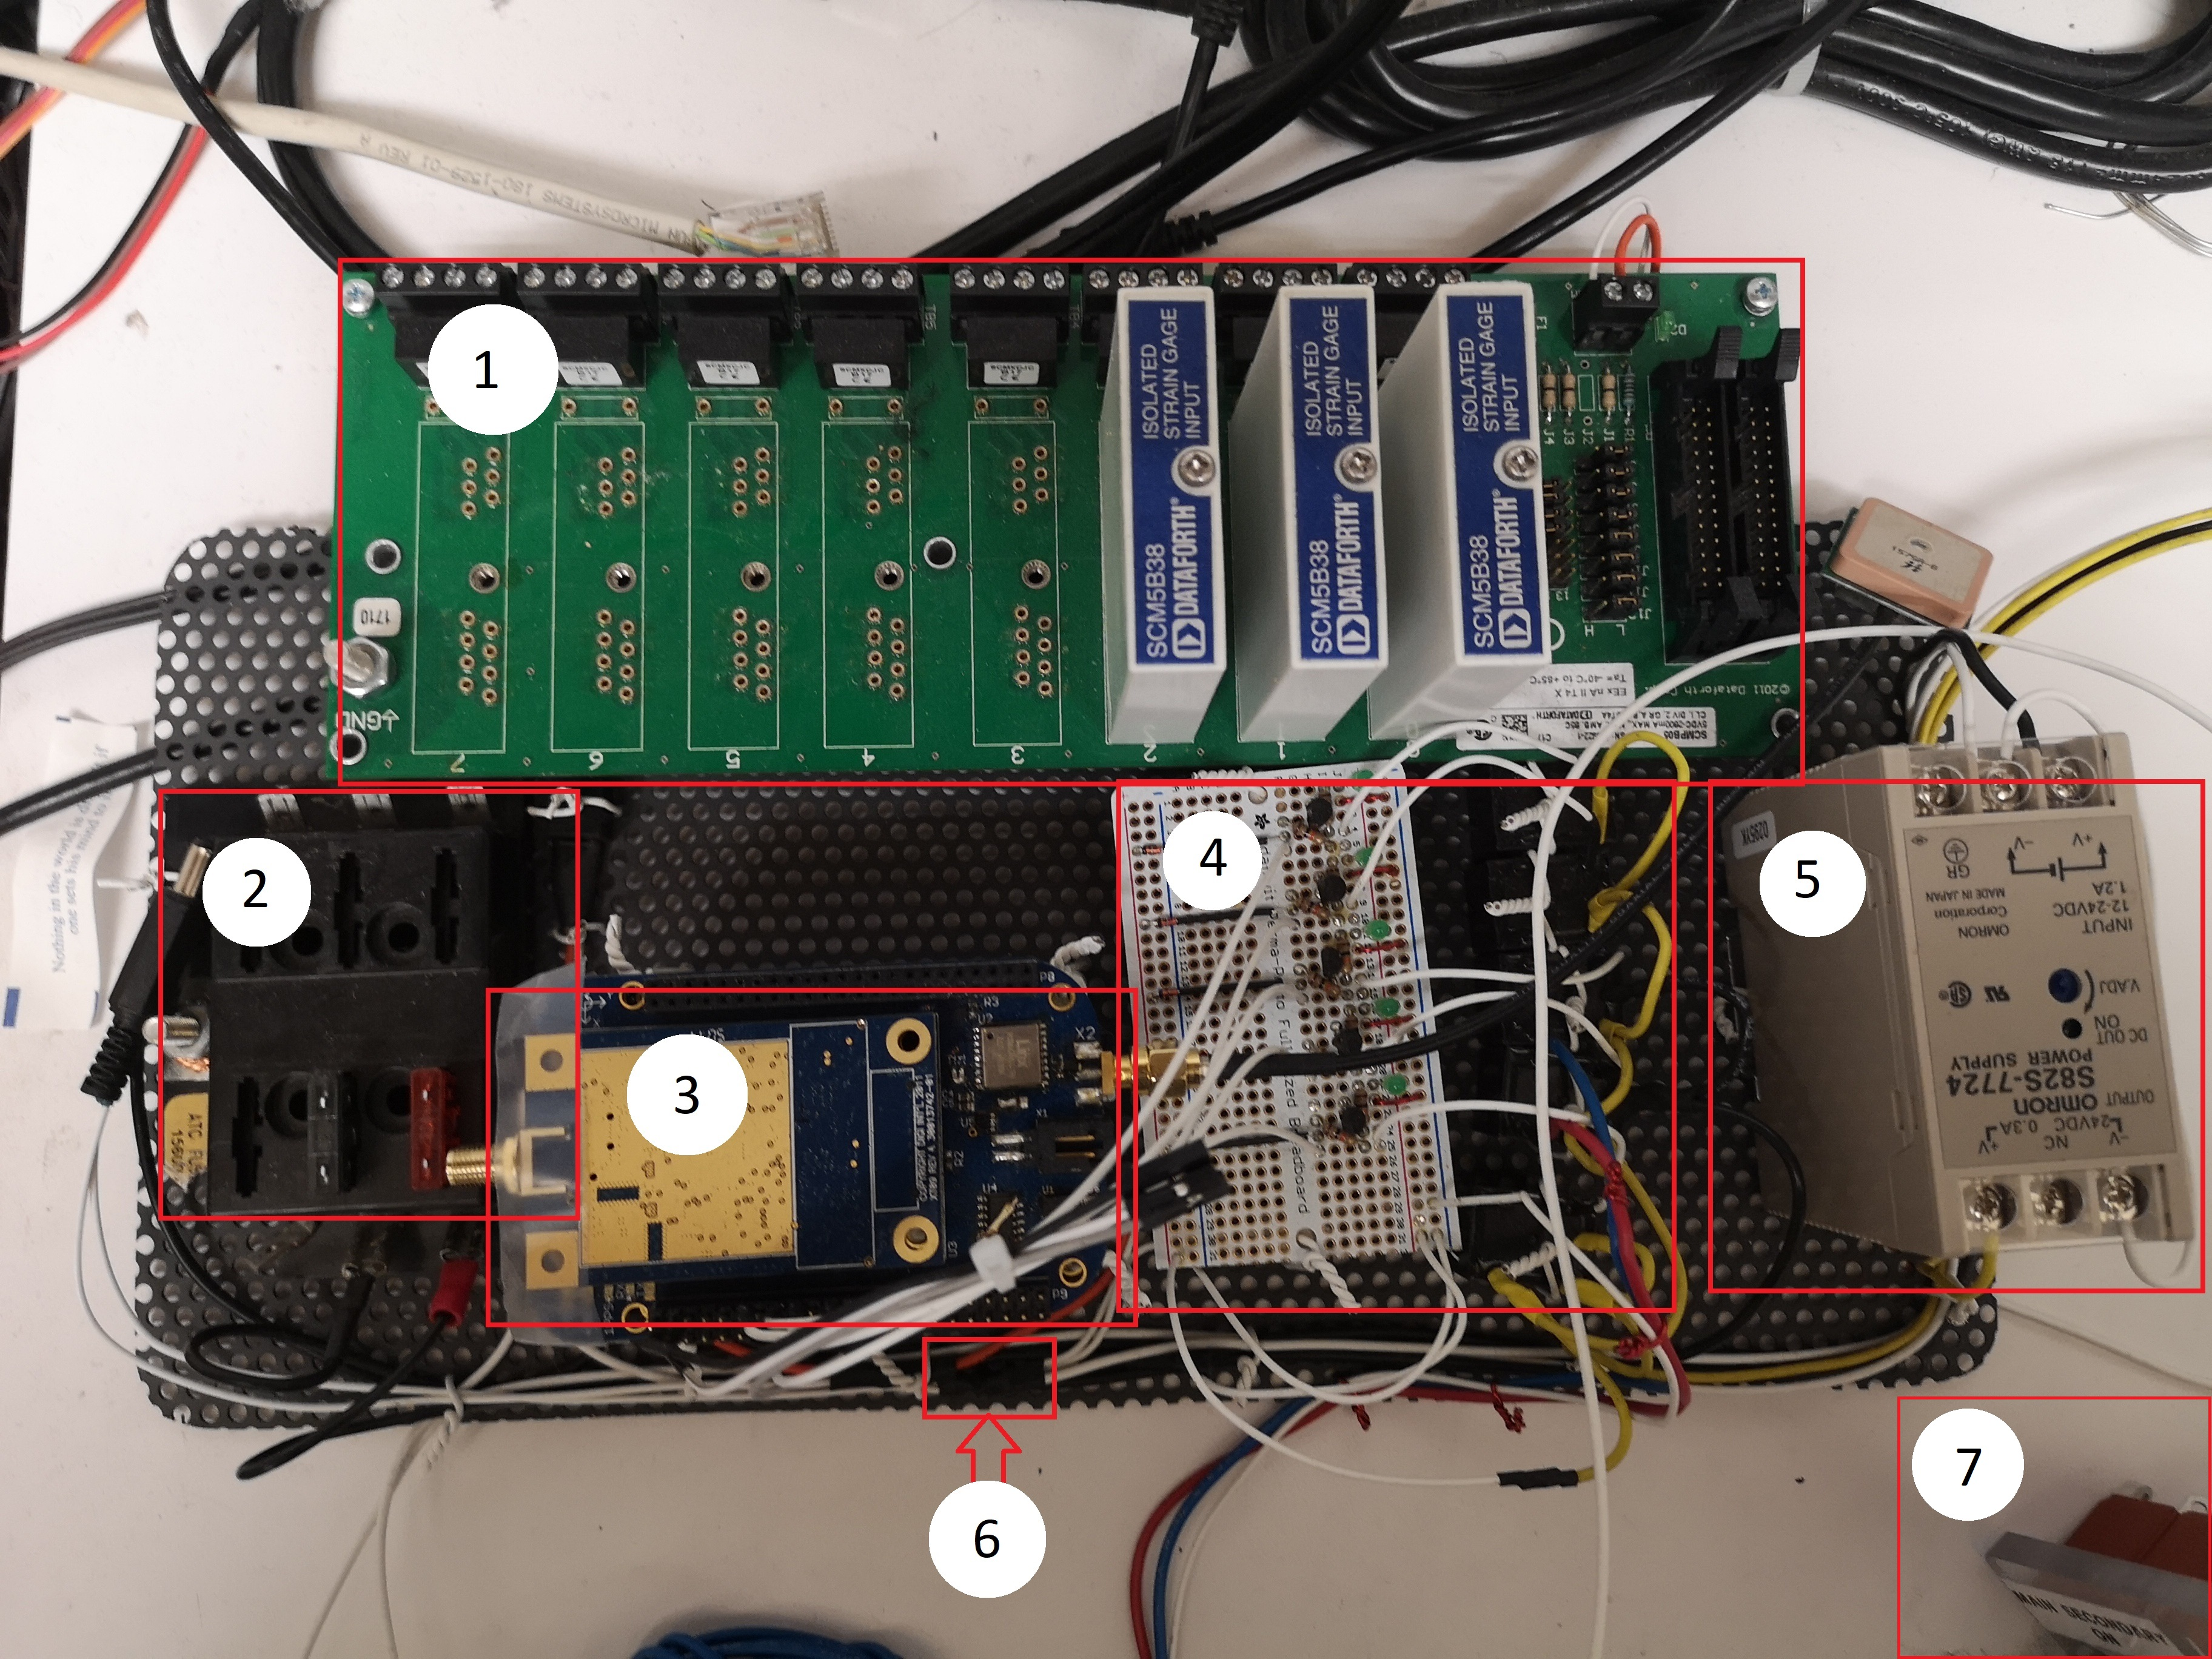
\includegraphics[width=7in]{EI00002_overview.jpg}

1. DAQ board. Allows for pressure transducers and other resistive measurement devices to be converted to a usable analog signal. Used with the National Instruments ADC (USB-6000).

2 Fuses. Provides separate fuses to parts of the system. Namely, one fuse to drive high-load circuitry (ignition and solenoids) and one to drive the remaining system.

3. Beaglebone Black Stack. The main computational stack that will be tested and programmed.

4. Relays and Relay-Drivers. A temporary installment that allows the Beaglebones' GPIO pins to directly drive a high load through a relay.

5. DC-DC 24V Step-up Converter. A DIN-rail device that will step up the battery voltage (~12V) to the a higher 24V used by the relays (I bought the wrong ones).

6. DC-DC 5V Power Regulator. A through hole 5V step mode power regulator to provide 5V power to various systems.

7. Power Switches for main and secondary power.

\begin{sidewaysfigure} % couldn't quite get this figure set up right
	\section{Circuitry}
	\centering
	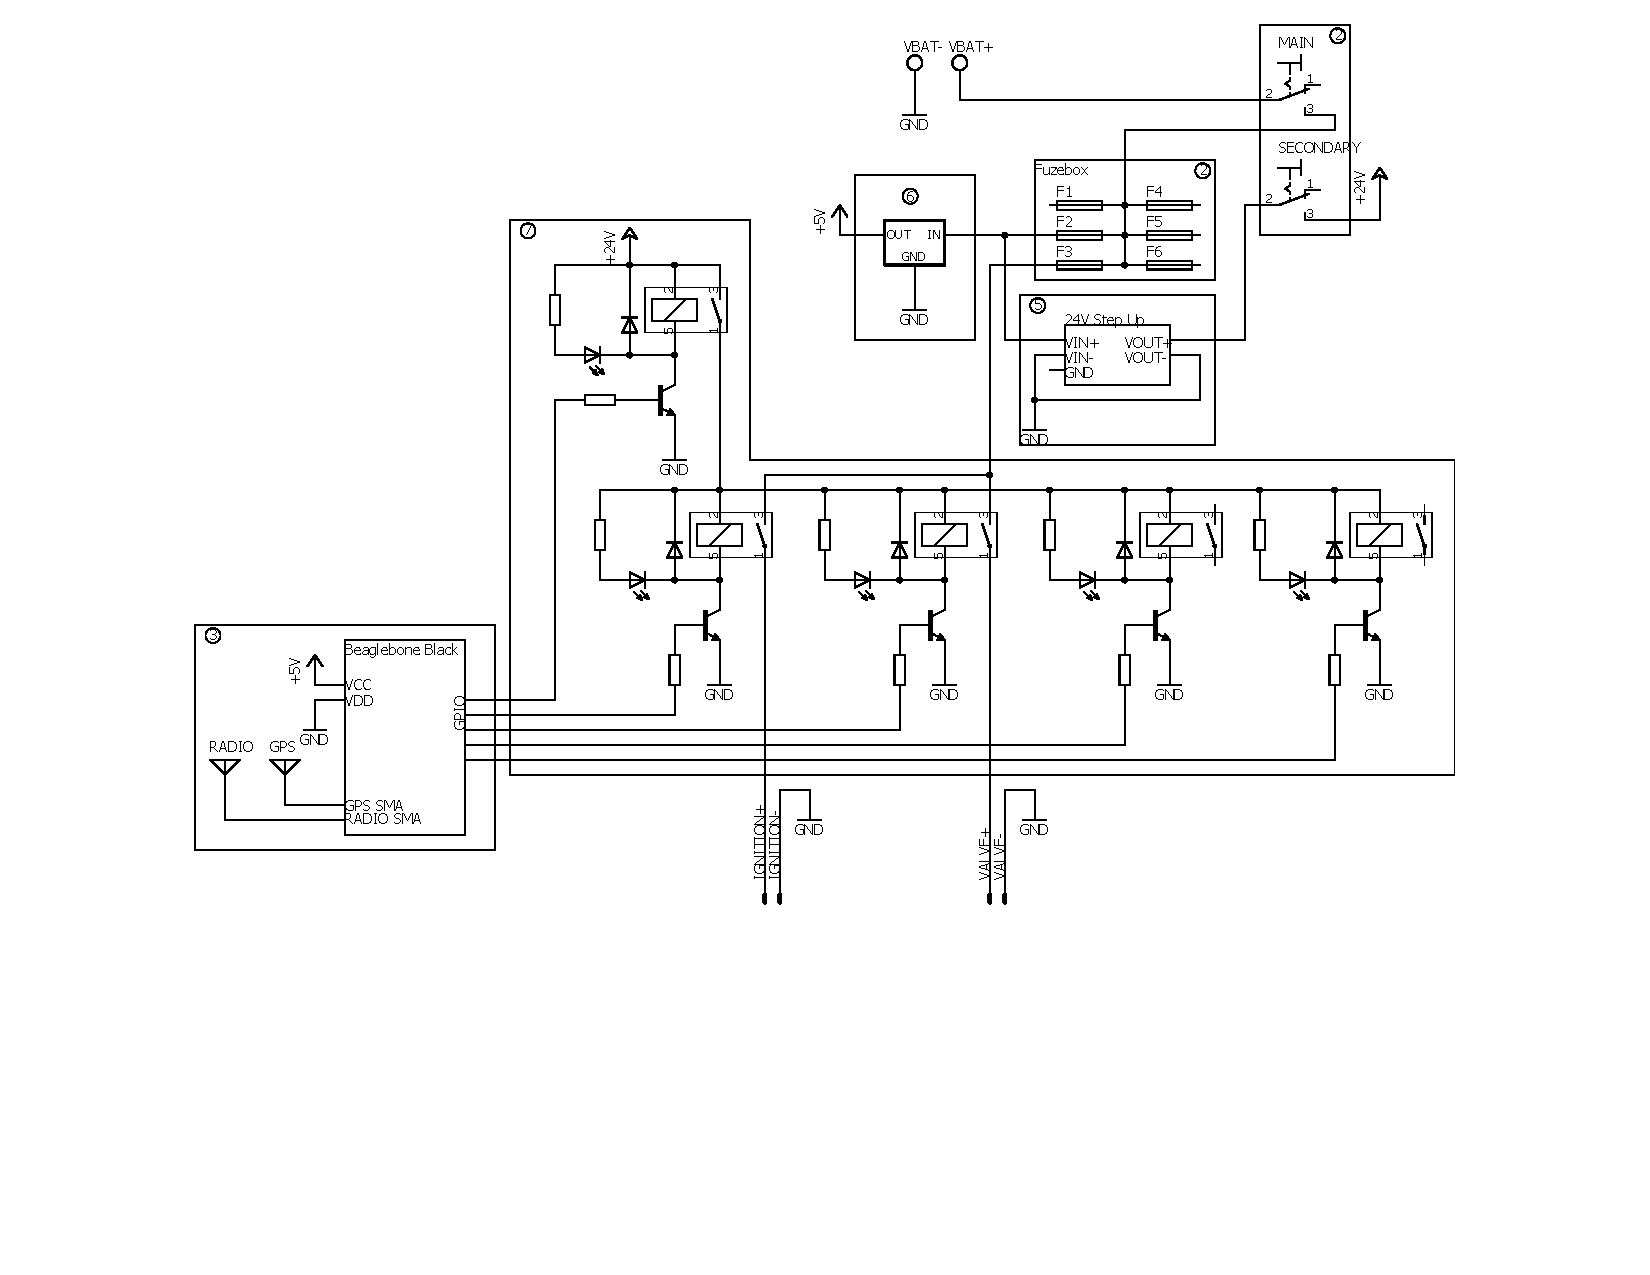
\includegraphics[width=10in]{EI00002_schematic.pdf} %angle=270, origin=c,
\end{sidewaysfigure}

\newpage
\section{Usage guide}
The test bench as it is currently is built to allow for actuation of a solenoid valve and an ignition coil, with the ability to add more high-power devices to the empty relays. It also provides signal conditioners for 2 force transducers and a pressure transducer.

To utilize the relays, the corresponding GPIO pin on the Beaglebone has to be driven high (or low, I don't remember). However, the first relay is meant as an enable for the remaining relays (see circuit diagram above) to allow for a safety interlock. In addition, the switch labeled SECONDARY must be enabled to allow for relay actuation to allow for manual override.\\
NOTE: When using the relays, make sure to set the pin mode to OUTPUT (i.e. run the script BEFORE turning on SECONDARY power) as a floating output may cause false triggers.

To utilize the signal conditioners, attach the National Instruments ADC to a computer running LabVIEW (namely the Japanese "still better than a mac" laptop). Run the LabVIEW program on that computer to start recording data.

\section{Additional notes}
The two fuses in the fuse box are rated loosely to protect the remaining circuitry. The higher rated fuse is meant to provide power to high-power devices (Ignition \& solenoid). The lower rated fuse provides power to the rest of the system.
Note that these fuses have not been tested, and a short on the ignition coil will cause all systems to crash.

\textbf{CAUTION:} All information contained in this documentation may be inaccurate or wrong. The test bench is not meant to be a final device and is built crudely at best.

\textbf{DO NOT USE IN CRITICAL APLICATIONS}

% End of document
%**********************************************************************
\end{document}